
% Section: EVALUATION
\section{Performance Evaluation}
\label{sec__dist_auctioneer_evaluation}

We have evaluated the implementations of the allocator for double and standard auctions proposed in \Cref{sec__dist_auctioneer_instances}.
The implementations of all the remaining blocks are as suggested in \Cref{sec__distrib_auctioneer_protocol_implementation}: 
we use the rational consensus algorithm proposed in~\cite{Afek2014} in the implementation of the bid agreement, 
while the input validation and data transfer blocks are implemented as simple broadcasts, 
and the common coin is implemented using the scheme from~\cite{Abraham2013}. 
For these implementations to be $k$-resilient equilibria, we need $m>2k$. 
This is a requirement of the rational consensus algorithm. 

Our goal is to assess the overhead of the distributed protocol, when compared to a purely centralised solution,
in the case the allocation algorithm is not parallelisable, 
and to assess the potential benefits from parallelisation when computationally expensive allocation algorithms are used. 
For that purpose, we measure performance gains for different levels $p$ of parallelism, where $p = \lfloor m/(k+1) \rfloor$ is the maximum level of parallelism for each possible $k$ and $p=1$ represents the sequential execution by a trusted auctioneer.
We consider a fixed number of $m=8$ providers in the auctions,
but we vary the number of providers that execute each protocol.

\subsection{Hardware/Software Setup}

In order to obtain a meaningful evaluation of our approach, we have resorted to a prototype implementation on realistic hardware and software environment and deployed it in an experimental testbed for community networks, namely on nodes of the Guifi.net, one of the largest community networks in the world~\cite{ClommunityTestbed}. 
We were given access to 4 different nodes of the experimental testbed, 2 machines in Barcelona (UPC Campus), and one machine each in Barcelona (Hangar) and in Taradell, Spain.
When doing tests executed by more than 4 providers we have instantiated 
multiple VMs in each nodes, ensuring that each VM is allocated a different CPU. 
The machines are Intel Core i7-3770 3.40GHz CPU with 16 GB RAM and 1 TB hard disk, running Proxmox virtualisation engine. 
Our experiment runs in OpenVZ containers with Debian 7 x86 1 CPU, 2 GB RAM, and 10 GB storage. 
We have implemented the framework in Python, using PyPy for speed reasons, 
and used \O{}MQ~\cite{ZeroMQ} as the messaging library for the communication.

We have set up a single node that acts as a client, and generates input for all the $n$ users.
This client node sends the requests to the $m$ providers, and receives the results back from all of them.
The values for running time presented in the plots capture the time from when the inputs are generated at this client node,
till the time it receives the results from all the experiment instances.
We run the experiments for 100 rounds, and plot the average values in the graphs.

\subsection{Double Auction Deployment}

We have used an experimental set up similar to~\cite{Zheng2014Star}, with some slight modifications suitable to our use case.
In both the experiments, the double and standard auction, 
the bids by the users are uniformly distributed in the range $[0.75, 1.25]$,
and the requested bandwidth resource is uniformly distributed in the range $(0, 1]$.
We vary the capacity of the providers depending upon the overall bandwidth required, and scale it using a random factor in $[0.5, 1.5]$ so as to consider both the cases where providers lack the capacity to satisfy all the requests, and where the providers have excess capacity.
The providers have a unit cost of bandwidth uniformly distributed in the range $(0, 1]$.

%% FIGURE
\begin{figure}[tbp]
	\centering
	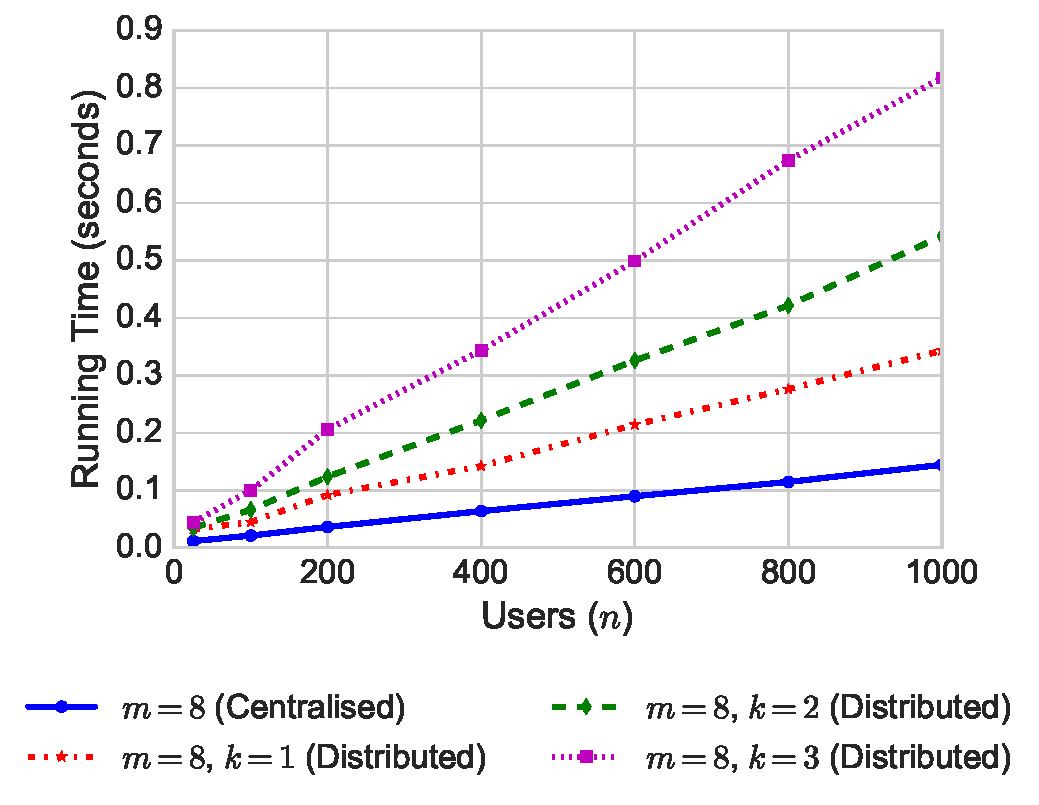
\includegraphics[width=0.65\columnwidth,keepaspectratio]{time-double-auction}
	\caption{Running time for double auction}
	\label{fig:double-auction-time}
\end{figure}

Figure~\ref{fig:double-auction-time} shows the running time for the double auction algorithm (\Cref{sec:instances-double-auction}) 
as a function of the number of users, for up to 1000 users. 
This algorithm has little computational overhead. 
It is not easily parallelisable but, as it can be observed from the figure, this is irrelevant as the distributed version is dominated by the communication time. 
Also, the communication overhead increases as the number of users increases, since more data has to be exchanged between the providers. 
The figure shows the values obtained for the centralised approach and for the distributed implementation using different values of $k$
and corresponding minimum required number of providers out of a total of 8 involved in the execution, namely, $3$ providers when $k=1$, $5$ when $k=2$, and $8$ when $k=3$. 
Even when 8 providers and 1000 users are used, the 
distributed implementation finishes in less than a second which is perfectly 
acceptable because normally these auctions need to run with reasonable intervals between them.

\subsection{Standard Auction Deployment}

We fix the number of providers to $m=8$ and vary the maximum degree of parallelisation 
by taking $p$ to be $1$, $2$, and $4$, corresponding to a centralised execution, $k=3$, and $k=1$, respectively.
Figure~\ref{fig:standard-auction-time} shows the running time for the standard 
auction (\Cref{sec:instances-vcg}) as a function of the number of users, for up to 125 users.
The capacity of the providers is based on the overall bandwidth required at that provider in the bids submitted by the users, and scaled down using a random factor in $[0, 0.25]$, so roughly no more than a quarter of the users win the bids. 
For higher values of $n$, the algorithm~\cite{Zhang2015Truthful} can take in the order of hours to complete, 
which is expected as its computational complexity is $\approx \mathcal{O}(mn^9(\frac{1}{\epsilon})^2)$ for $n$ users and $m$ providers, though it provides better guarantees for social welfare than other alternatives.

Figure~\ref{fig:standard-auction-time} shows that the running time in general grows quickly as $n$ increases, and there is sharp rise in the running time for values of $n$ close to 100.
This is because the running time of the algorithm~\cite{Zhang2015Truthful} is 
a function of the feasible allocation space (which can grow exponentially in the worst case) of the resource allocation problem.
Therefore, the communication and coordination overhead is not significant when compared to the running time of the allocation algorithm. 
On the contrary, the overheads involved in distributing the inputs and aggregating the results from the providers are easily offset by the gains due to parallelisation in this case. 
In Figure~\ref{fig:standard-auction-time},  we can observe significant performance 
gains in the distributed case, for $p=2$ and $p=4$ (i.e., for $k=3$ and $k=1$ respectively). 
For instance, when 8 providers are available and $k=1$ the distributed implementation
takes around 100 seconds while the serial implementation takes around 400 seconds. 
This indicates that our approach allows for scaling the allocation algorithm, 
given that when the network grows more providers also become available.

\begin{figure}[tbp]
	\centering
	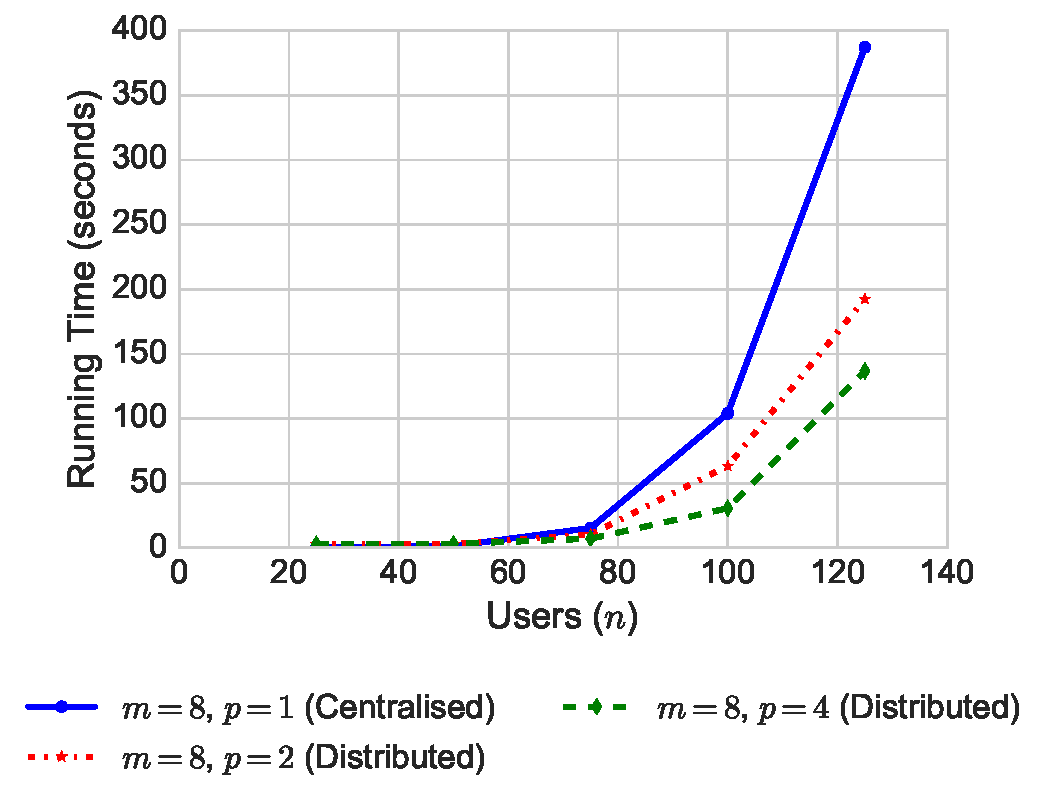
\includegraphics[width=0.65\columnwidth,keepaspectratio]{time-vcg}
	\caption{Running time for standard auction}
	\label{fig:standard-auction-time}
\end{figure}
